% Intended LaTeX compiler: pdflatex
\documentclass[10pt,a4paper,UTF8]{article}
\usepackage{zclorg}
\author{张朝龙}
\date{}
\title{学习Python Doc第六天: 输入和输出}
\hypersetup{
 pdfauthor={张朝龙},
 pdftitle={学习Python Doc第六天: 输入和输出},
 pdfkeywords={},
 pdfsubject={},
 pdfcreator={Emacs 25.0.50.1 (Org mode 9.0.5)}, 
 pdflang={English}}
\begin{document}

\maketitle
\tableofcontents
\titlepic{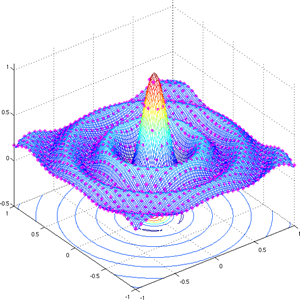
\includegraphics[scale=0.25]{../../img/sinc.PNG}}
一个程序的输出可以有多种呈现方式:1)通过屏幕打印;2)通过写入文件。今天我们来探讨这两种方法。

\section{多种多样的输出格式}
\label{sec:orgd236dd1}


像在 \texttt{C} 语言中一样, \texttt{Python} 也提供了样式繁多的输出格式。在 \texttt{Python} 中你可以自己控制输出格式,可以通过 \texttt{str.format()} 这个方法实现。

在 \texttt{Python} 中有两种方式实现值到字符串的转换:  \texttt{repr()} 和 \texttt{str()} 。 \texttt{repr()} 函数生成解释器可读的格式; \texttt{str()} 生成人类可读的格式。(看Python Tutorial的这段文字的时候,有想打人的冲动,写的非常零散。本以为英文文档应该会好一些,现在对Python的官方手册质量不敢恭维,) 直接看代码:

\lstset{language=Python,label= ,caption= ,captionpos=b,numbers=none}
\begin{lstlisting}
In [25]: s = 'hello, world.'

In [26]: str(s)
Out[26]: 
'hello, world.'

In [27]: s
Out[27]: 
'hello, world.'

In [28]: str(1/7)
Out[34]: 
'0.14285714285714285'

In [35]: x = 10 * 3.25

In [50]: y= 200*200

In [66]: s = 'the value of x is ' + repr(x) + ', and y is ' + repr(y) + '...'

In [123]: print(s)
the value of x is 32.5, and y is 40000...

In [128]: #the repr() of a string adds string quotes and backslashes:

In [160]: hello = 'hello world\n'

In [168]: hellos = repr(hello)

In [172]: print(hellos)
'hello world\n'

In [173]: # the argument to repr() may be any python objects:

In [189]: repr((x,y,('spam','eggs')))
Out[215]: 
"(32.5, 40000, ('spam', 'eggs'))"
\end{lstlisting}

接下来给出两种输出平方表和立方表的方法:
\lstset{language=Python,label= ,caption= ,captionpos=b,numbers=none}
\begin{lstlisting}
for x in range(1,11):
    print(repr(x).rjust(2), repr(x*x).rjust(3),end = ' ')
    print(repr(x*x*x).rjust(4))
\end{lstlisting}

输出为:
\begin{verbatim}
In [218]:
 1   1    1
 2   4    8
 3   9   27
 4  16   64
 5  25  125
 6  36  216
 7  49  343
 8  64  512
 9  81  729
10 100 1000
\end{verbatim}
另一种方法为:
\lstset{language=Python,label= ,caption= ,captionpos=b,numbers=none}
\begin{lstlisting}
for x in range(1,11):
    print('{0:2d} {1:3d} {2:4d}'.format(x,x*x,x*x*x))
\end{lstlisting}
输出同上一种方法。

注意:在第一种方法中,每一列后都有一个空格,这个空格是 \texttt{print()} 自动加上去的, \texttt{print()} 总是在它的参数中加空格。第一种方法演示了字符对象的 \texttt{str.rjust()} 方法。 \texttt{str.rjust()} 实现了右对齐。举一反三,存在 \texttt{str.ljust} 和 \texttt{str.center()} . 还有另外一个方法 \texttt{str.zfill()} 这个方法在一串数值前面填零。看代码:

\lstset{language=Python,label= ,caption= ,captionpos=b,numbers=none}
\begin{lstlisting}
In [220]: '12'.zfill(6)
Out[233]: 
'000012'

In [234]: 'abc'.zfill(6)
Out[241]: 
'000abc'

In [242]: '-abc'.zfill(6)
Out[262]: 
'-00abc'

In [263]: '-45'.zfill(6)
Out[283]: 
'-00045'
\end{lstlisting}

可以看出 \texttt{str.zfill} 把 \texttt{.} 之前的字符当做有符号数值字符。

基本的 \texttt{str.format()} 使用方法是:
\begin{verbatim}
>>> print('We are the {} who say "{}!"'.format('knights', 'Ni'))
We are the knights who say "Ni!"
\end{verbatim}

使用大括号代表待输入的参数,输入参数通过 \texttt{.format} 提供。可以通过在大括号中填入数字指定 \texttt{.format} 后的字符串填入的位置。

\lstset{language=Python,label= ,caption= ,captionpos=b,numbers=none}
\begin{lstlisting}
In [284]: print('{0} and {1}'.format('spam','egg'))
spam and egg

In [302]: print('{1} and {0}'.format('spam','egg'))
egg and spam

In [303]: print('{2} and {0}'.format('spam','egg'))
---------------------------------------------------------------------------
IndexError       Traceback (most recent call last)
<ipython-input-303-f5413a9d7179> in <module>()
----> 1 print('{2} and {0}'.format('spam','egg'))

IndexError: tuple index out of range
\end{lstlisting}
可以看到也有数组越界问题存在。

可以在 \texttt{print()} 中使用关键字。比如:
\lstset{language=Python,label= ,caption= ,captionpos=b,numbers=none}
\begin{lstlisting}
In [304]: print('This {food} is {adjestive}.'.format(food='spam',adjective='absolutely horrible'))
---------------------------------------------------------------------------
KeyError            Traceback (most recent call last)
<ipython-input-389-9f9f624a721c> in <module>()
----> 1 print('This {food} is {adjestive}.'.format(food='spam',adjective='absolutely horrible'))

KeyError: 'adjestive'

In [390]: print('This {food} is {adjective}.'.format(food='spam',adjective='absolutely horrible'))
This spam is absolutely horrible.
\end{lstlisting}

注意关键词的对应。也可以组合以上两种方法:
\lstset{language=Python,label= ,caption= ,captionpos=b,numbers=none}
\begin{lstlisting}
In [396]: print('The story of {0},{1},and {other}'.format('Bill','Manfred',other='Georg'))
The story of Bill,Manfred,and Georg
\end{lstlisting}

通过 \texttt{:} 来指定显示格式。
\lstset{language=Python,label= ,caption= ,captionpos=b,numbers=none}
\begin{lstlisting}
In [472]: print('pi is {0:.3f}'.format(math.pi))
pi is 3.142
\end{lstlisting}
在 \texttt{:} 之后跟上一个整数可以指定最小的显示宽度,这在美化表格显示方面非常有用。
\begin{verbatim}
table = {'Sjoerd': 4127,'Jack':4098,'Dcab':7678}
for name,phone in table.items():
    print('{0:10} ==> {1:10d}'.format(name,phone) )
\end{verbatim}
输出为:
\begin{verbatim}
In [560]: 
Sjoerd     ==>       4127
Jack       ==>       4098
Dcab       ==>       7678
\end{verbatim}
\subsection{之前的字符格式化方式}
\label{sec:org202d00b}


\texttt{\%} 字符在较老的Python版本中用来做字符串格式化,其格式化过程与 \texttt{sprintf()} 函数差不多。

\begin{verbatim}
In [565]: print('pi is %5.3f' % math.pi)
pi is 3.142
\end{verbatim}
\section{文件的读写}
\label{sec:orgafd3fe2}


\texttt{open()} 返回一个文件对象,最经常的实用方式是 \texttt{open(filename,mode)}

第一个参数是文件名字,第二个是文件的读写模式可选的选项有:
\begin{enumerate}
\item \texttt{r} 只读
\item \texttt{w} 只写,同名文件会被覆盖。
\item \texttt{a} 打开文件,写在文件最后边。
\item \texttt{r+} 读写。
\end{enumerate}

默认情况下 \texttt{mode} 参数的值是 \texttt{r} 。

通常,文件是作为文本进行编辑的,也就是说有指定的文本编码格式。 \texttt{b} 是二进制编码。如果没有指定编码格式则文本的编码格式依操作系统平台而定。

文件的常用方法有: 
\begin{enumerate}
\item \texttt{f.read()} 读出文件内容。
\item \texttt{f.readline()} 读出文件的一行。
\item \texttt{f.write(string)} 向文件中写入。
\item \texttt{f.seek(5)} 找到文件的第6行。
\item \texttt{f.close()} 关闭文件。
\end{enumerate}
\subsection{使用 \texttt{json}}
\label{sec:org760b4d3}


字符串可以很容易的读写,数值就麻烦了点儿。因为 \texttt{read()} 函数只返回字符串。如果读出 \texttt{'123'} 还需要使用 \texttt{int()} 来返回真实的数值。碰上复杂的数据类型,操作就更麻烦了。

万幸, \texttt{Python} 使用 \texttt{JSON} (JavaScript Object Notation)来作为数据保存格式, \texttt{JSON} 是一种广为使用的数据交换格式。。 Python有处理 \texttt{JSON} 的标准库 \texttt{json} 。这个库可以方便的层次化保存数据,把这些数据保存成字符串(这个过程叫做 \texttt{serializing} );也可以方便的把这些字符创变回数值( 这个过程叫做 \texttt{deserializing}  ).  

关于 \texttt{JSON} 的介绍就到这里,以后用到了再来补充。
\end{document}
